%
% wanderweg.tex -- Wanderweg als Extremalproblem mit Nebenbedingung
%
% (c) 2021 Prof Dr Andreas Müller, OST Ostschweizer Fachhochschule
%
\bgroup
\begin{frame}[t]
\setlength{\abovedisplayskip}{5pt}
\setlength{\belowdisplayskip}{5pt}
\frametitle{Höchster Punkt einer Wanderung}
\vspace*{-3pt}
\begin{center}
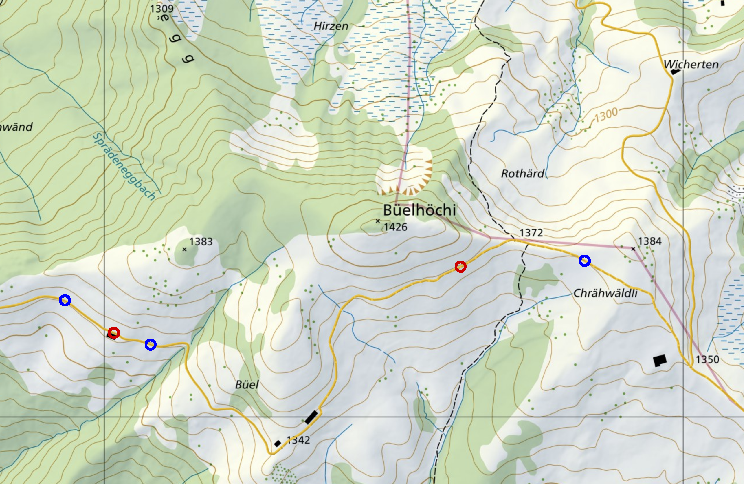
\includegraphics[width=11.6cm]{../../buch/chapters/010-fuvar/images/karteextremum.pdf}
\end{center}
\end{frame}
\egroup
